% Synchronized to r49561
\marklabel{sec:openvpn}{
  \section{OpenVPN - VPN Support}}
\hyphenation{Open-VPN}

\sloppy

As of version 2.1.5 package OpenVPN is part of fli4l.

\wichtig{For using OpenVPN over the Internet a flatrate or billing 
  based on data volume is a must have! If the fli4l router is 
  powered on the connection will never be hung up because a small 
  amount of data is permanently transferred by OpenVPN. Using a 
  VPN Tunnel over the Internet thus can cause high online costs. The 
  same is applying for an ISDN connection being used for OpenVPN.}

Besides OpenVPN another VPN package exists: OPT\_PoPToP
(see opt-database \altlink{http://www.fli4l.de/download/zusatzpakete/}).

Deciding which VPN solution to use is driven by security and function 
concerns. No advices on security of the different packages are given 
by the team. In unsure, see

Linux-Magazine January 2004

\altlink{http://diswww.mit.edu/bloom-picayune/crypto/14238}

\altlink{http://sites.inka.de/bigred/archive/cipe-l/2003-09/msg00263.html}

Concerning functionality a clear advice can be given to use 
OpenVPN which outperforms both CIPE and poptop here. OpenVPN 
supports tunnel mode, bridge mode, data compression and is more solid 
than CIPE on a fli4l router. OpenVPN has a Windows version to be used 
as of Windows 2000. Only disadvantages against CIPE are the sheer size 
in opt archive and missing OpenVPN support for fli4l version 2.0.x.

\subsection{OpenVPN - Introductive Example}

To introduce you to OpenVPN's configuration at first a small example. 
Two networks that both use a fli4l router shall be connected over the 
Internet. OpenVPN establishes an encrypted tunnel on both fli4l routers 
to let computers from both nets communicate with each other. The configuration 
variables shown in picture \ref{fig:tunnel} are used for this purpose.

  \begin{figure}[htbp]
    \centering
    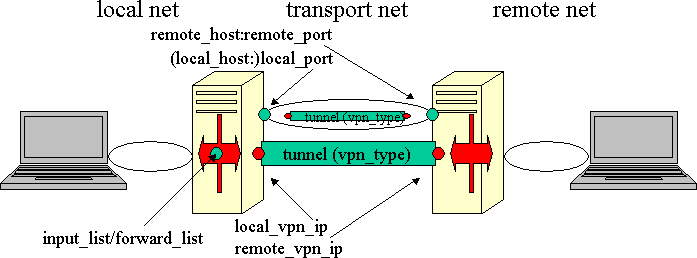
\includegraphics[width=\columnwidth]{openvpn-sample}
    \caption{VPN configuration example --- tunnel between two routers}
    \label{fig:tunnel}
  \end{figure}

  \begin{description}

  \item [local net, remote net] represent the two nets to be connected 
  by the tunnel. They have to be in different TCP/IP ranges and should 
  have different non interfering net masks. The settings from 
  \jump{IPNETx}{\var{IP\_NET\_x}} in both routers base.txt configuration 
  files hence have to be different. Thus it is not possible to connect 
  two nets over a tunnel that both use IP range 192.168.6.0/24.

  \item [transport net] The transport network consists of two elements:

  \begin{itemize}

  \item the connection between two OpenVPN daemons, described by 
  \emph{\smalljump{OPENVPNxREMOTEHOST}{remote\_host}:\smalljump{OPENVPNxREMOTEPORT}{remote\_port}}
  and \emph{(\smalljump{OPENVPNxLOCALHOST}{local\_host}:)\smalljump{OPENVPNxLOCALPORT}{local\_port}}. 
  This is an equivalent to the OpenVPN settings in \var{OPENVPN\_x\_REMOTE\_HOST},
  \var{OPENVPN\_x\_REMOTE\_PORT}, \var{OPENVPN\_x\_LOCAL\_HOST} and
  \var{OPENVPN\_x\_LOCAL\_PORT}.

  \item and a tunnel over which the connection between the two OpenVPN-Daemons 
  is established, described by 
  \emph{\smalljump{OPENVPNxLOCALVPNIP}{local\_vpn\_ip}/\smalljump{OPENVPNxREMOTEVPNIP}{remote\_vpn\_ip}}. 
  This again is an equivalent to the OpenVPN settings in 
  \var{OPENVPN\_x\_LOCAL\_VPN\_IP} and \var{OPENVPN\_x\_REMOTE\_VPN\_IP}. 
  Both VPN IP addresses have be set to values of non existent nets on 
  both routers.

  \end{itemize}

  \item [\smalljump{OPENVPNxPFINPUTN}{input\_list},
  \smalljump{OPENVPNxPFFORWARDN}{forward\_list}] Packets that should be 
  sent over this tunnel have to pass the packet filter at first. It will 
  only allow ICMP messages (i.e. ping) as the default which can be used to 
  test the tunnel. Everythihng else has to be allowed explicitly. 
  In the simplest case this is done by

\begin{example}
\begin{verbatim}
OPENVPN_x_PF_INPUT_POLICY='ACCEPT'
OPENVPN_x_PF_FORWARD_POLICY='ACCEPT'
\end{verbatim}
\end{example}

  \achtung{Plese note that \glqq{}accepting\grqq{} a complete VPN 
  connection is very critical in terms of security. Better use the tmpl: 
  syntax of the packet filter to only allow those services needed.}

  \end{description}

No more settings are required for a simple VPN tunnel. All other 
configuration handles extended functions or special use cases. You 
should use those after establishing a working tunnel with this minimal 
configuration. 

\subsection{OpenVPN - Configuration}

Because of the complexity of OpenVPN we start by explaining settings 
required for any VPN connection. Don't try extended configurations 
for OpenVPN before establishing a connection with minimal settings.

\begin{description}

\config{OPT\_OPENVPN}{OPT\_OPENVPN}{OPTOPENVPN}

  Default: \var{OPT\_OPENVPN='no'}

  \var{'yes'} activates package OpenVPN. 
  \var{'no'} deactivates package OpenVPN completely.

\config{OPENVPN\_N}{OPENVPN\_N}{OPENVPNN}

  Default: \var{OPENVPN\_N='0'}

  How many OpenVPN configurations are active in the configuration file?

\config{OPENVPN\_x\_REMOTE\_HOST}{OPENVPN\_x\_REMOTE\_HOST}{OPENVPNxREMOTEHOST}

  Default: \var{OPENVPN\_x\_REMOTE\_HOST=''}

  IP address or DNS address of the remote OpenVPN. For a \jump{roadwarrior}{Roadwarrior} 
  this line has to be completely omitted. If omitted OpenVPN waits for connection 
  establishment and doesn't try to connect by itself.

\config{OPENVPN\_x\_REMOTE\_HOST\_N}{OPENVPN\_x\_REMOTE\_HOST\_N}{OPENVPNxREMOTEHOSTN}

  Default: \var{OPENVPN\_x\_REMOTE\_HOST\_N='0'}

  Using dynamic DNS services is not alsways 100\% reliable. You may simply 
  use two ore more of those DynDNS services to register your current IP 
  address with all of them at the same time. To enable OpenVPN to go through 
  the whole DynDNS names a list of \emph{additional} DNS names has to be set. 
  By the help of \var{OPENVPN\_x\_REMOTE\_HOST} OpenVPN will try to contact 
  these addresses in random order. Hence \var{OPENVPN\_x\_REMOTE\_HOST} 
  has to exist and be configured correctly!

\config{OPENVPN\_x\_REMOTE\_HOST\_x}{OPENVPN\_x\_REMOTE\_HOST\_x}{OPENVPNxREMOTEHOSTx}

  Default: \var{OPENVPN\_x\_REMOTE\_HOST\_x=''}

  Same description as above applies here
  \jump{OPENVPNxREMOTEHOST}{\var{OPENVPN\_x\_REMOTE\_HOST}}.

\config{OPENVPN\_x\_REMOTE\_PORT}{OPENVPN\_x\_REMOTE\_PORT}{OPENVPNxREMOTEPORT}

  Default: \var{OPENVPN\_x\_REMOTE\_PORT=''}

  Each OpenVPN connection does need an unused port address on the fli4l 
  router. It is adviced to use ports above 10000 for those are not 
  commonly used. If configuring a connection for a remote station with 
  dynamically changing IP address that has no DynDNS address omit 
  this entry as well as \var{OPENVPN\_x\_REMOTE\_HOST}.

\config{OPENVPN\_x\_LOCAL\_HOST}{OPENVPN\_x\_LOCAL\_HOST}{OPENVPNxLOCALHOST}

  Default: \var{OPENVPN\_x\_LOCAL\_HOST=''}

  Specifies to what IP address OpenVPN will bind. For connections over the 
  Internet this entry should be completely omitted. If an address is set here 
  OpenVPN will only listen for incoming traffic on this IP. If you want to 
  secure a WLAN connection you should set the IP address of fli4l's WLAN 
  interface card here.

\config{OPENVPN\_x\_LOCAL\_PORT}{OPENVPN\_x\_LOCAL\_PORT}{OPENVPNxLOCALPORT}

  Default: \var{OPENVPN\_x\_LOCAL\_PORT=''}

  Specifies the port number the local OpenVPN daemon will listen to.
  For each OpenVPN connection you need a reserved port that only can 
  be used by this connection. Other software on the router is not 
  allowed to use this port. \var{OPENVPN\_x\_REMOTE\_PORT} and 
  \var{OPENVPN\_x\_LOCAL\_PORT} of each OpenVPN connection have to match! 
  If setting \var{OPENVPN\_x\_REMOTE\_PORT='10111'} on one side of the tunnel 
  \var{OPENVPN\_x\_LOCAL\_PORT='10111'} \emph{has to be set} on the other 
  side as well.
  
  Again: It is very important to match these settings to the according 
  remote OpenVPN station otherwise a connection is not possible between 
  OpenVPN partners.

  To enable OpenVPN to listen to incoming connections OpenVPN itself opens the 
  ports in the packet filter set in \var{OPENVPN\_x\_LOCAL\_PORT}. If this is 
  not your wish then you may change this behavior in 
  \jump{OPENVPNDEFAULTOPENOVPNPORT}{\var{OPENVPN\_DEFAULT\_OPEN\_OVPNPORT}}. 
  It is \emph{not} necessary to set \var{OPENVPN\_DEFAULT\_OPEN\_OVPNPORT='yes'} 
  because this is the default behavior!

  OpenVPN does not work with ports lower than 1025. If i.e. OpenVPN should 
  work as a tcp4- or tcp6-server on port 443 (https port) you have to forward this 
  port via the packet filter to a port above 1024. If i.e. OpenVPN is 
  listening on port 5555 and port 443 should be forwarded there 
  \var{PF\_PREROUTING} has to be set like this:

\begin{example}
\begin{verbatim}
PF_PREROUTING_5='tmpl:https dynamic REDIRECT:5555'
\end{verbatim}
\end{example}

\config{OPENVPN\_x\_SECRET}{OPENVPN\_x\_SECRET}{OPENVPNxSECRET}

  Default: \var{OPENVPN\_x\_SECRET=''}

  OpenVPN needs a keyfile for encrypting an OpenVPN connection. This 
  keyfile can be generated unter Windows or Linux by OpenVPN itself. 
  Beginners may install OpenVPN's Windows software or use OpenVPN's
  WebGUI. If you do not want to use OpenVPN under Windows but only 
  generate the needed keyfiles it is enough to install 
  \emph{OpenVPN User-Space Components}, \emph{OpenSSL DDLs}, 
  \emph{OpenSSL Utilities}, \emph{Add OpenVPN to PATH} and 
  \emph{Add Shortcuts to OpenVPN}. With choosing 
  \emph{Generate a static OpenVPN key} from the OpenVPN start menu 
  the keyfiles needed can be generated. At the end the message 
  \glqq{}Randomly generated 2048 bit key written to
  \var{C:/Program files/OpenVPN/config/key.txt}\grqq{} will appear. 
  The file \var{key.txt} is the one we need. Copy this file into 
  the directory \var{$<$config$>$/etc/openvpn} and change its name 
  \var{key.txt} to something more meaningful. Keyfiles can also be 
  generated automatically by the fli4l router if you set 
  \var{OPENVPN\_CREATE\_SECRET} to \var{'yes'} and reboot fli4l. 
  If configuring OpenVPN for the first time enter all data in the 
  config file and either set 
  \jump{OPENVPNDEFAULTCREATESECRET}{\var{OPENVPN\_DEFAULT\_CREATE\_SECRET}}
  to \var{'yes'} if one keyfile should be used for all connections or 
  if a keyfile for only one connection should be generated set  
  \var{OPENVPN\_x\_CREATE\_SECRET} to \var{'yes'}. After boot of the 
  fli4l router one or more keyfiles will be created automatically 
  and saved to \var{/etc/openvpn} with the name specified.  
  Keyfile(s) can be copied via scp or other medias. After creation 
  of keyfiles change the setting back to 'no' and build a new boot 
  media for fli4l with the configuration and keyfiles you just created. 
  If you forget to change 'yes' to 'no' fli4l will generate new keyfiles 
  with each reboot but no OpenVPN daemon will be started and thus no tunnels 
  can be established. If you set \var{OPENVPN\_x\_CREATE\_SECRET} to
  \var{'webgui'} you can use the web interface to generate keyfiles. Use 
  OpenVPN's WebGUI in detail view for connections and choose 'Keymanagement'.
  For reference see \ref{sec:openvpn_gui}

  Hint: By executing 
  \begin{verbatim}
      openvpn --genkey --secret <filename>
  \end{verbatim}
  you can generate a keyfile by hand via fli4l's console.

  Keyfiles have to be copied to the directory \var{$<$config$>$/etc/openvpn} 
  as seen in the following picture. The file name of the keyfiles without 
  path has to set in \var{OPENVPN\_x\_SECRET}. In this way keyfiles will 
  be copied to the opt-archive while creating the boot media.

  \begin{figure}[htbp]
    \centering
    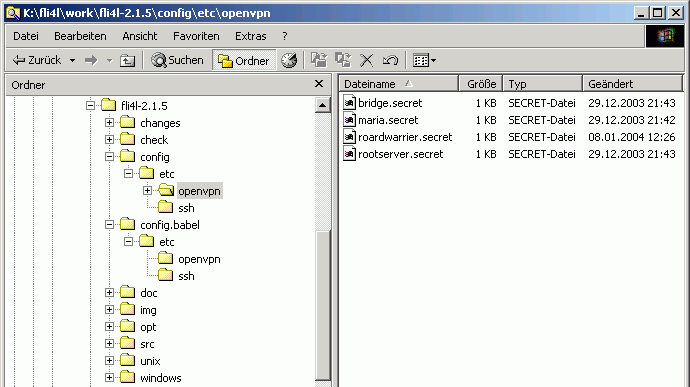
\includegraphics[width=\columnwidth]{config_etc_openvpn}
    \caption{fli4l config directory with OpenVPN *.secret files}
    \label{fig:config_etc_openvpn}
  \end{figure}

\config{OPENVPN\_x\_TYPE}{OPENVPN\_x\_TYPE}{OPENVPNxTYPE}

  Default: \var{OPENVPN\_x\_TYPE=''}

  An OpenVPN connection either can be used as a tunnel or as a bridge. 
  Through an OpenVPN tunnel only IP traffic can be routed. A bridge 
  transfers ethernet frames i.e. not only IP traffic but also IPX or 
  NetBEUI or else. For using OpenVPN to transfer ethernet frames package 
  advanced\_networking is needed in addition. Please note that a bridge 
  over a DSL line can be really slow!

\end{description}

\subsection{OpenVPN - Bridge configuration}

  For using OpenVPN as a bridge the following entries are valid. Please 
  note that when using a bridge over the Internet broadcast traffic 
  uses already a rather high bandwidth without any real data being transferred.

  Remember that the following settings are only valid if for this connection 
  \jump{OPENVPNxTYPE}{\var{OPENVPN\_x\_TYPE}} is set to \var{'bridge'}! A 
  configured bridge from package advanced\_networking to which the VPN 
  connection can bind is needed additionally.

\begin{description}

\config{OPENVPN\_x\_BRIDGE}{OPENVPN\_x\_BRIDGE}{OPENVPNxBRIDGE}

  Default: \var{OPENVPN\_x\_BRIDGE=''}

  Holds the name of the bridge this OpenVPN connection should bind to. If 
  \var{BRIDGE\_DEV\_x\_NAME='cuj-br'} is given and the OpenVPN connection 
  should bind to that bridge \var{'cuj-br'} has to be set in accordance.

\config{OPENVPN\_x\_BRIDGE\_COST}{OPENVPN\_x\_BRIDGE\_COST}{OPENVPNxBRIDGECOST}

  Default: \var{OPENVPN\_x\_BRIDGE\_COST=''}

  If using spanning tree protocol (STP, see \altlink{http://de.wikipedia.org/wiki/Spanning_Tree} 
  or documentation for package advanced\_networking) you can specify the connection 
  costs here.
  
\config{OPENVPN\_x\_BRIDGE\_PRIORITY}{OPENVPN\_x\_BRIDGE\_PRIORITY}{OPENVPNxBRIDGEPRIORITY}

  Default: \var{OPENVPN\_x\_BRIDGE\_PRIORITY=''}

  If using STP (spanning tree protocol, see \altlink{http://de.wikipedia.org/wiki/Spanning_Tree} 
  or documentation for package advanced\_networking) you can specify connection 
  priority here.

\end{description}

\subsection{OpenVPN - Tunnel configuration}

\begin{description}

\config{OPENVPN\_x\_REMOTE\_VPN\_IP}{OPENVPN\_x\_REMOTE\_VPN\_IP}{OPENVPNxREMOTEVPNIP}

  Default: \var{OPENVPN\_x\_REMOTE\_VPN\_IP=''}

  This setting is only valid if \jump{OPENVPNxTYPE}{\var{OPENVPN\_x\_TYPE}} 
  is set to \var{'tunnel'} for this OpenVPN connection!

  VPN IP address of the OpenVPN remote station. VPN IP addresses are needed only 
  for routing and can be chosen nearly free. The following restrictions apply:

\begin{itemize}

\item IP address may not be used in local network and thus can't be in the subnet of the fli4l router.

\item IP address may not be used for any local network device.

\item IP address may not belong to any network routed by \var{IP\_ROUTE\_x}.

\item IP address may not belong to any network routed by \var{ISDN\_CIRC\_ROUTE\_x}.

\item IP address may not belong to any network routed by \var{CIPE\_ROUTE\_x}.

\item IP address may not belong to any network routed by \var{OPENVPN\_ROUTE\_x}.

\item IP address may not belong to any network used or routed by fli4l in any other way.

\end{itemize}

  As you see VPN IP addresses can't be used anywhere else. Before beginning to configure 
  OpenVPN you should look for an unused net in both local and remote address ranges. 
  It should belong to private address ranges (see \altlink{http://ftp.univie.ac.at/netinfo/rfc/rfc1597.txt}).

\config{OPENVPN\_x\_LOCAL\_VPN\_IP}{OPENVPN\_x\_LOCAL\_VPN\_IP}{OPENVPNxLOCALVPNIP}

  Default: \var{OPENVPN\_x\_LOCAL\_VPN\_IP=''}

  This setting is only valid if \jump{OPENVPNxTYPE}{\var{OPENVPN\_x\_TYPE}} 
  is set to \var{'tunnel'} for this OpenVPN connection.

  IP address for the local OpenVPN device tunX. Same restrictions as in 
  \jump{OPENVPNxREMOTEVPNIP}{\var{OPENVPN\_x\_REMOTE\_VPN\_IP}}
  apply here.

  By the way, it is possible to use the same IP address as in \var{OPENVPN\_x\_LOCAL\_VPN\_IP} 
  for all local OpenVPN connections. This enables a host host to use the same IP address 
  in all VPNs. Packet filter rules are drastically easier to configure this way.
  
\config{OPENVPN\_x\_IPV6}{OPENVPN\_x\_IPV6}{OPENVPNIPV6}

  Default: \var{OPENVPN\_x\_IPV6='no'}
  
  This enables native IPv6 support in OpenVPN. Consider this as an experimental feature because 
  of the code being brandnew. Of course OPT\_IPV6 has to be activated and configured as well then. 
  For \var{OPENVPN\_x\_IPV6='no'} and/or \var{OPT\_IPV6='no'} all relevant variables are ignored. 
  
  ATTENTION!!! These settings are not checked for overlapping with other parts of the 
  configuration! This applies to \var{OPENVPN\_x\_LOCAL\_VPN\_IPV6},
  \var{OPENVPN\_x\_REMOTE\_VPN\_IPV6} and \var{OPENVPN\_x\_ROUTE\_x}.
  
\config{OPENVPN\_x\_REMOTE\_VPN\_IPV6}{OPENVPN\_x\_REMOTE\_VPN\_IPV6}{OPENVPNxREMOTEVPNIPV6}

  Default: \var{OPENVPN\_x\_REMOTE\_VPN\_IPV6=''}
  
  For IPv6 the same restrictions apply as for \jump{OPENVPNxREMOTEVPNIP}{\var{OPENVPN\_x\_REMOTE\_VPN\_IP}}.
  
  \begin{example}
  \begin{verbatim}
    OPENVPN_X_REMOTE_IPV6='FD00::1'
  \end{verbatim}
  \end{example}

\config{OPENVPN\_x\_LOCAL\_VPN\_IPV6}{OPENVPN\_x\_LOCAL\_VPN\_IPV6}{OPENVPNxLOCALVPNIPV6}

  Default: \var{OPENVPN\_x\_LOCAL\_VPN\_IPV6=''}
  
  For IPv6 applies the same as for \jump{OPENVPNxLOCALVPNIP}{\var{OPENVPN\_x\_LOCAL\_VPN\_IP}}.
  If no subnet is set /64 will be used as a default.
  
  \begin{example}
  \begin{verbatim}
    OPENVPN_X_LOCAL_IPV6='FD00::2/112'
  \end{verbatim}
  \end{example}

\config{OPENVPN\_x\_ROUTE\_N}{OPENVPN\_x\_ROUTE\_N}{OPENVPNxROUTEN}

  Default: \var{OPENVPN\_x\_ROUTE\_N=''}

  This setting is only valid if \jump{OPENVPNxTYPE}{\var{OPENVPN\_x\_TYPE}} 
  is set to \var{'tunnel'} for this OpenVPN connection.

  Routes are being set automatically by OpenVPN when starting up. 
  Up to 50 nets can be routed over a single OpenVPN connection. 
  For every net to be routed a valid \var{OPENVPN\_x\_ROUTE\_x} entry
  must be created.

  Please note that the packet filter rules necessary have to be set manually in 
  \var{OPENVPN\_PF\_FORWARD\_x} \var{OPENVPN\_PF\_INPUT\_x} res.
  \var{OPENVPN\_PF6\_FORWARD\_x} \var{OPENVPN\_PF6\_INPUT\_x}.
  OpenVPN only allows ICMP over a VPN connection and denies all other 
  data traffic. Details can be found at 
  \jump{OPENVPNxPFINPUTN}{\var{OPENVPN\_x\_PF\_INPUT\_N}} and
  \jump{OPENVPNxPFFORWARDN}{\var{OPENVPN\_x\_PF\_FORWARD\_N}} res.
  at
  \jump{OPENVPNxPF6INPUTN}{\var{OPENVPN\_x\_PF6\_INPUT\_N}} and
  \jump{OPENVPNxPF6FORWARDN}{\var{OPENVPN\_x\_PF6\_FORWARD\_N}}.
  
  For very special configurations it is possible to start scripts
  e.g. to enable policy-based routing. The scripts need to be stored
  in the directory \texttt{config/etc/openvpn} and have to be named
  as follows:
  
  
\begin{example}
  <name>-<time>
\end{example}

  ``name'' stands for the name of the OpenVPN connection
  (\var{OPENVPN\_x\_NAME}). For ``time''  the following
   choices for the execution of the scripts are available:

  \begin{itemize}
    \item [up-pre] Before establishing the OpenVPN connection.
    \item [up-post] After establishing the OpenVPN connection.
    \item [down-pre] Before ending the OpenVPN connection.
    \item [down-post] After ending the OpenVPN connection.
    \item [route-up-pre] Before setting the OpenVPN routes.
    \item [route-up-post] After setting the OpenVPN routes.
    \item [route-down-pre] Before deleting the OpenVPN routes.
    \item [route-down-post] After deleting the OpenVPN routes.
  \end{itemize}

  To start a script for the connection \var{OPENVPN\_x\_NAME='maria'}
  after setting the routes its name has to be \texttt{maria-route-up-post}
  and it has to be created in the directory \texttt{config/etc/openvpn}.

\config{OPENVPN\_x\_ROUTE\_x}{OPENVPN\_x\_ROUTE\_x}{OPENVPNxROUTEx}

  Default: \var{OPENVPN\_x\_ROUTE\_x=''}

  Specify the nets to be reached over the OpenVPN remote station here.
  If on the remote side i.e. the nets 192.168.33.0/24 and 172.18.0.0/16 
  can be reached and should be accessed through the OpenVPN tunnel both 
  of them have to be entered under \var{OPENVPN\_x\_ROUTE\_x}. 
  Host routes (\var{/32}) may be set here as well.

  If the default route should be reached through an OpenVPN tunnel specifiy 
  0.0.0.0/0 res. ::/0 for IPv6 and an optional flag as routes here. 
  For IPv6 routes OPT\_IPv6 has to be activated, local and remote IPv6 
  addresses for the tunnel have to be set and OPENVPN\_x\_IPV6 
  must be 'yes'. OpenVPN has several alternative ways to set a default route
  which can be chosen by a flag. Each method has its own advantages and 
  disadvantages. At the moment the following flags are supported:

\begin{itemize}
\item [local] The \emph{local} flag should be chosen if the OpenVPN 
	      remote station is located in a subnet that can be reached 
	      directly by the fli4l router. This may be the case for example 
	      for an OPENVPN default route over WLAN.
\item [def1] With this flag two new routes 0.0.0.0/1 and 128.0.0.0/1 will 
	     be defined in addition to a host route to the OpenVPN remote 
	     station. This routes act as default routes for the complete 
	     (encrypted) traffic to the OpenVPN remote station (which can 
	     be reached over the host route).
\end{itemize}

  If omitting the optional flag OpenVPN will choose the method of setting 
  default routes. Methods will be picked by the OpenVPN version. At the moment 
  \emph{local} is the default advised.

\begin{example}
\begin{verbatim}
OPENVPN_1_ROUTE_N='3'
OPENVPN_1_ROUTE_1='192.168.33.0/24'
OPENVPN_1_ROUTE_2='172.18.0.0/16'
OPENVPN_1_ROUTE_3='2001:db8:/32'
\end{verbatim}
\end{example}

\end{description}

\subsubsection{OpenVPN - Delegation Of DNS and Reverse-DNS}

\begin{description}

\config{OPENVPN\_x\_DOMAIN}{OPENVPN\_x\_DOMAIN}{OPENVPNxDOMAIN}

  Default: \var{OPENVPN\_x\_DOMAIN=''}

  This parameter sets the remote domain. The variable can hold multiple domains 
  which have to be separated by spaces then. If only this parameter is set (without 
  mentioning of an additional DNS server) it will be assumed that a DNS server is listening 
  on the IP of the other end of the tunnel (see \jump{OPENVPNxREMOTEVPNIP}{\var{OPENVPN\_x\_REMOTE\_VPN\_IP}}).
  On the remote router incoming DNS queries have to allowed in this case.
  (i.e. via \var{OPENVPN\_x\_INPUT\_y='tmpl:dns ACCEPT'})

\config{OPENVPN\_x\_ROUTE\_x\_DOMAIN}{OPENVPN\_x\_ROUTE\_x\_DOMAIN}{OPENVPNxROUTExDOMAIN}

  Default: \var{OPENVPN\_x\_ROUTE\_x\_DOMAIN=''}

  Different subnets can have different domains assigned. Per \var{OPENVPN\_x\_ROUTE\_y} one 
  according domain can be configured. If a \var{OPENVPN\_x\_ROUTE\_y\_DNSIP} exists for the domain, 
  it will be used, else the one set at \var{OPENVPN\_x\_DNSIP}. The effect is the same as 
  with \var{OPENVPN\_x\_DOMAIN} but this method allows better documentation.

\config{OPENVPN\_x\_DNSIP}{OPENVPN\_x\_DNSIP}{OPENVPNxDNSIP}

  Default: \var{OPENVPN\_x\_DNSIP=''}

  If the tunnel end point is not the appropriate DNS server set the IP of the appropriate one here.
  If this is empty the one at \jump{OPENVPNxREMOTEVPNIP}{\var{OPENVPN\_x\_REMOTE\_VPN\_IP}} will 
  be used.

\config{OPENVPN\_x\_ROUTE\_x\_DNSIP}{OPENVPN\_x\_ROUTE\_x\_DNSIP}{OPENVPNxROUTExDNSIP}

  Default: \var{OPENVPN\_x\_ROUTE\_x\_DNSIP=''}

  Multiple subnets routed can also have different DNS servers - define one per 
  \jump{OPENVPNxROUTEx}{\var{OPENVPN\_x\_ROUTE\_x}} here.

\end{description}

\subsection{Expert Settings}

Almost all settings described in this chapter are optional and should only be 
changed if the OpenVPN connection is working but should be optimized 
(for example by the use of another key length).

Except \var{OPENVPN\_DEFAULT\_CIPHER} and \var{OPENVPN\_DEFAULT\_DIGEST},
all settings in \var{OPENVPN\_DEFAULT\_} are optional. This means they 
don't have to be written in the config file. If an entry is missing in 
openvpn.txt the OpenVPN start script will use the default value described 
here. If you don't want to change this defaults do not write them to the 
\texttt{openvpn.txt} config file!

\subsubsection{General Settings}

\begin{description}

\config{OPENVPN\_DEFAULT\_CIPHER}{OPENVPN\_DEFAULT\_CIPHER}{OPENVPNDEFAULTCIPHER}

  Enter an encryption method here. Currently the encryption methods
  in table~\ref{openvpn:ciphers} are supported.

  \begin{table}[!ht]
    \centering
    \caption{Available encryption methods in OpenVPN}
    \label{openvpn:ciphers}
    \begin{tabular}{|p{4cm}|r|r|l|}
      \hline
      Abbreviation	& nominal key length & effective key length & rating \\
      \hline
      none             &   0 Bit &   0 Bit & not safe \\
      DES-CBC          &  56 Bit &  56 Bit & not safe \\
      DES-EDE-CBC      & 112 Bit &  80 Bit & not safe \\
      DES-EDE3-CBC     & 168 Bit & 112 Bit & not safe \\
      DESX-CBC         & 184 Bit & 119 Bit & not safe \\
      RC2-40-CBC       &  40 Bit &  40 Bit & not safe \\
      RC2-64-CBC       &  64 Bit &  64 Bit & not safe \\
      RC2-CBC          & 128 Bit & 128 Bit & not safe \\
      BF-CBC           & 128 Bit & 128 Bit & safe \\
      CAST5-CBC        & 128 Bit & 128 Bit & safe \\
      AES-128-CBC      & 128 Bit & 128 Bit & safe \\
      AES-192-CBC      & 192 Bit & 192 Bit & safe \\
      AES-256-CBC      & 256 Bit & 256 Bit & safe \\
      CAMELLIA-128-CBC & 128 Bit & 128 Bit & safe \\
      CAMELLIA-192-CBC & 192 Bit & 192 Bit & safe \\
      CAMELLIA-256-CBC & 256 Bit & 256 Bit & safe \\
      SEED-CBC         & 128 Bit & 128 Bit & safe \\
      \hline
    \end{tabular}
  \end{table}

  \wichtig{This variable has \emph{no} default! You have to select
  an algorithm. If in doubt, please choose
  \begin{itemize}
  \item ``AES-128-CBC'', if you can use hardware support for it
        (siehe Paket ``hwsupp''), or
  \item ``AES-256-CBC'', if you have a fast CPU (1 GHz or
        more), or
  \item ``BF-CBC'' in all other cases.
  \end{itemize}}

  In former fli4l versions this variable's default was ``BF-CBC''.

\config{OPENVPN\_DEFAULT\_COMPRESS}{OPENVPN\_DEFAULT\_COMPRESS}{OPENVPNDEFAULTCOMPRESS}

  Default: \var{OPENVPN\_DEFAULT\_COMPRESS='yes'}

  OpenVPN uses adaptive LZO data compression to enlarge the bandwidth 
  of a connection. Adaptive means OpenVPN recognizes by itself when i.e. 
  already compressed zip files are sent over an OpenVPN connection. In 
  such case data compression will be switched off until data is sent that 
  will benefit from data compression. There is nearly no cause for 
  deactivating data compression because this enlarges bandwidth at nearly 
  no cost. Only disadvantage of data compression is a small increase of 
  latency by some milliseconds. For online games via VPN which need 
  a ''good'' ping, i.e. low latency it may be wise to deactivate 
  data compression. 
  
\config{OPENVPN\_DEFAULT\_CREATE\_SECRET}{OPENVPN\_DEFAULT\_CREATE\_SECRET}{OPENVPNDEFAULTCREATESECRET}

  Default: \var{OPENVPN\_DEFAULT\_CREATE\_SECRET='no'}

  This setting will cause OpenVPN to automatically generate keyfiles on 
  boot of the fli4l router. An OpenVPN connection won't be started then. 
  For details see \jump{OPENVPNxSECRET}{\var{OPENVPN\_x\_SECRET}}.

\config{OPENVPN\_DEFAULT\_DIGEST}{OPENVPN\_DEFAULT\_DIGEST}{OPENVPNDEFAULTDIGEST}

  Enter a checksum calculation method here. Currently
  the methods in table~\ref{openvpn:digests} are supported.

  \begin{table}[!ht]
    \centering
    \caption{Checksum calculation methods available in OpenVPN}
    \label{openvpn:digests}
    \begin{tabular}{|p{4cm}|r|l|}
      \hline
      Abbreviation	& Checksum length & Rating\\
      \hline
      none             &   0 Bit & not safe \\
      MD4              & 128 Bit & not safe \\
      RSA-MD4          & 128 Bit & not safe \\
      MD5              & 128 Bit & not safe \\
      RSA-MD5          & 128 Bit & not safe \\
      MDC2             & 128 Bit & safe \\
      RSA-MDC2         & 128 Bit & safe \\
      SHA              & 160 Bit & not safe \\
      RSA-SHA          & 160 Bit & not safe \\
      SHA1             & 160 Bit & not safe \\
      RSA-SHA1         & 160 Bit & not safe \\
      DSA-SHA          & 160 Bit & not safe \\
      DSA-SHA1-old     & 160 Bit & not safe \\
      DSA-SHA1         & 160 Bit & not safe \\
      RSA-SHA1-2       & 160 Bit & not safe \\
      DSA              & 160 Bit & not safe \\
      RIPEMD160        & 160 Bit & safe \\
      RSA-RIPEMD160    & 160 Bit & safe \\
      ecdsa-with-SHA1  & 160 Bit & safe \\
      SHA224           & 224 Bit & safe \\
      RSA-SHA224       & 224 Bit & safe \\
      SHA256           & 256 Bit & safe \\
      RSA-SHA256       & 256 Bit & safe \\
      SHA384           & 384 Bit & safe \\
      RSA-SHA384       & 384 Bit & safe \\
      SHA512           & 512 Bit & safe \\
      RSA-SHA512       & 512 Bit & safe \\
      whirlpool        & 512 Bit & safe \\
      \hline
    \end{tabular}
  \end{table}

  \wichtig{This variable has \emph{no} default! You have to select an
  algorithm. If in doubt, choose
  \begin{itemize}
  \item ``whirlpool'', if you have a fast CPU (1 GHz or more),
        or
  \item ``SHA256'' in other cases.
  \end{itemize}}

  In former fli4l versions this variable's default was ``SHA1''.

\config{OPENVPN\_DEFAULT\_FLOAT}{OPENVPN\_DEFAULT\_FLOAT}{OPENVPNDEFAULTFLOAT}

  Default: \var{OPENVPN\_DEFAULT\_FLOAT='yes'}

  OpenVPN remote stations that use DynDNS addresses can change their IP address 
  at any time. To make OpenVPN accept this changed IP address set 
  \var{OPENVPN\_DEFAULT\_FLOAT} to \var{'yes'}. If \var{'no'} is set 
  changing of an IP address is not allowed. This only makes sense with WLAN 
  connections or connections to remote stations with static IP addresses 
  (i.e. some provider's root servers). This setting can be superseded be a 
  per connection setting as all other \var{OPENVPN\_DEFAULT\_} settings can. 

\config{OPENVPN\_DEFAULT\_KEYSIZE}{OPENVPN\_DEFAULT\_KEYSIZE}{OPENVPNDEFAULTKEYSIZE}

  Default: \var{OPENVPN\_DEFAULT\_KEYSIZE=''}

  Keysize depends on the encryption method used. Only change this setting when 
  connecting to an OpenVPN remote station that does not use default settings 
  and which you have no influence on. If keysize can be determined by you this 
  value should stay empty. OpenVPN will use the optimal keysize for the 
  encryption method used then.

\config{OPENVPN\_DEFAULT\_OPEN\_OVPNPORT}{OPENVPN\_DEFAULT\_OPEN\_OVPNPORT}{OPENVPNDEFAULTOPENOVPNPORT}

  Default: \var{OPENVPN\_DEFAULT\_OPEN\_OVPNPORT='yes'}

  fli4l's packet filter rules have to be changed to enable OpenVPN connections. 
  For all TCP or UDP ports (see \var{OPENVPN\_x\_PROTOCOL}) OpenVPN should listen 
  on \jump{PFNEWCONFIG}{\var{PF\_INPUT\_x}} in base.txt has to be adapted. By 
  specifiying \var{'yes'} these packet filter rules will be generated 
  automatically. For some connections it may make sense to set \var{'no'} 
  and define the rules yourself.

\config{OPENVPN\_DEFAULT\_ALLOW\_ICMPPING}{OPENVPN\_DEFAULT\_ALLOW\_ICMPPING}{OPENVPNDEFAULTALLOWICMPPING}

  Default: \var{OPENVPN\_DEFAULT\_ALLOW\_ICMPPING='yes'}

  \var{'yes'} configures the packet filter for the connection to let 
  pass ping data packets. If there is no really good cause ICMP ping 
  should be allowed at any time. This setting is \emph{not} equivalent 
  to OpenVPN's ping option!

\config{OPENVPN\_DEFAULT\_PF\_INPUT\_LOG}{OPENVPN\_DEFAULT\_PF\_INPUT\_LOG}{OPENVPNDEFAULTPFINPUTLOG}

  Default: \var{OPENVPN\_DEFAULT\_PF\_INPUT\_LOG='BASE'}

  \var{'yes'} or \var{'no'} sets whether the packet filter should protocol 
  denied incoming packets for the VPN connection in the INPUT list or not. 
  By specifiying \var{'BASE'} the setting from \var{'PF\_INPUT\_LOG='} in 
  base.txt will be used.

\config{OPENVPN\_DEFAULT\_PF\_INPUT\_POLICY}{OPENVPN\_DEFAULT\_PF\_INPUT\_POLICY}{OPENVPNDEFAULTPFINPUTPOLICY}

  Default: \var{OPENVPN\_DEFAULT\_PF\_INPUT\_POLICY='REJECT'}

  This setting equals \jump{PFINPUTPOLICY}{\var{'PF\_INPUT\_POLICY}='}
  in base.txt. By specifiying \var{'BASE'} the setting from  \var{'PF\_INPUT\_POLICY='} 
  in base.txt will be used.
  
\config{OPENVPN\_DEFAULT\_PF\_FORWARD\_LOG}{OPENVPN\_DEFAULT\_PF\_FORWARD\_LOG}{OPENVPNDEFAULTPFFORWARDLOG}

  Default: \var{OPENVPN\_DEFAULT\_PF\_FORWARD\_LOG='BASE'}

  \var{'yes'} or \var{'no'} sets whether the packet filter should protocol 
  denied incoming packets for the VPN connection in the FORWARD list or not. 
  By specifiying \var{'BASE'} the setting from \var{'PF\_FORWARD\_LOG='} in 
  base.txt will be used.

\config{OPENVPN\_DEFAULT\_PF\_FORWARD\_POLICY}{OPENVPN\_DEFAULT\_PF\_FORWARD\_POLICY}{OPENVPNDEFAULTPFFORWARDPOLICY}

  Default: \var{OPENVPN\_DEFAULT\_PF\_FORWARD\_POLICY='REJECT'}

  This setting equals \jump{PFFORWARDPOLICY}{\var{'PF\_FORWARD\_POLICY='}} 
  in base.txt. By specifiying \var{'BASE'} the setting from \var{'PF\_FORWARD\_POLICY='} in 
  base.txt will be used.

\config{OPENVPN\_DEFAULT\_PING}{OPENVPN\_DEFAULT\_PING}{OPENVPNDEFAULTPING}

  Default: \var{OPENVPN\_DEFAULT\_PING='60'}

  To keep an established tunnel open and to recognize if the OpenVPN remote 
  station can still be reached an encrypted ping will be sent over the line 
  in the interval in seconds specified here. \var{'off'} does not send pings 
  over the line but only real user data.

\config{OPENVPN\_DEFAULT\_PING\_RESTART}{OPENVPN\_DEFAULT\_PING\_RESTART}{OPENVPNDEFAULTPINGRESTART}

  Default: \var{OPENVPN\_DEFAULT\_PING\_RESTART='180'}

  If in the time interval set here no ping or other data is transferred 
  succesfully the VPN connection concerned will be restarted. The value 
  in \var{OPENVPN\_DEFAULT\_PING\_RESTART} has to be greater than the 
  one in \var{OPENVPN\_DEFAULT\_PING}. \var{'off'} disables automatic 
  restart.

\config{OPENVPN\_DEFAULT\_RESOLV\_RETRY}{OPENVPN\_DEFAULT\_RESOLV\_RETRY}{OPENVPNDEFAULTRESOLVRETRY}

  Default: \var{OPENVPN\_DEFAULT\_RESOLV\_RETRY='infinite'}

  If \var{OPENVPN\_x\_REMOTE\_HOST} or \var{OPENVPN\_x\_LOCAL\_HOST} 
  holds DNS names instead of IP addresses they have to be resolved 
  to IP addresses when starting an OpenVPN connection. If this fails 
  OpenVPN will retry to resolve the DNS name for the timespan set here. 
  If this doesn't work within the time limit set here no OpenVPN 
  connection will be established. With \var{'infinite'} OpenVPN will 
  try forever to resolve the DNS name. Only change this setting if 
  if you know what you're doing!

\config{OPENVPN\_DEFAULT\_RESTART}{OPENVPN\_DEFAULT\_RESTART}{OPENVPNDEFAULTRESTART}

  Default: \var{OPENVPN\_DEFAULT\_RESTART='ip-up'}

  After disconnection of a tunnel an immedeate restart should be done 
  in order to keep disconnection time as small as possible. For all OpenVPN 
  connections made over dial-in lines like DSL or ISDN \var{'ip-up'} should 
  be specified here. \var{'never'} should be set instead for OpenVPN connections 
  over WLAN because of reconnection being independent of dial-ins. 
  For OpenVPN tunnels over an ISDN dial-in connection being established 
  with \var{ISDN\_CIRC\_x\_TYPE='raw'} \var{'raw-up'} has to be set here.

\config{OPENVPN\_DEFAULT\_PROTOCOL}{OPENVPN\_DEFAULT\_PROTOCOL}{OPENVPNDEFAULTPROTOCOL}

  Default: \var{OPENVPN\_DEFAULT\_PROTOCOL='udp4'}

  This variable sets which protocol should be used as default. UDP is a 
  a good choice normally but sometimes only TCP is allowed, which has a 
  remarkable overhead. 
  Possible values are \var{'udp4'}, \var{'udp6'}, \var{'tcp4-server'}, 
  \var{'tcp6-server'}, \var{'tcp4-client'} or \var{'tcp6-client'}.
  Settings \var{'tcp[46]-server'} or \var{'tcp[46]-client'} make only sense 
  if a VPN tunnel has to be established through a number of paket filters 
  or other tunnels. If no special case should be handled \emph{always} 
  use the default setting \var{'udp4'} or \var{'udp6'}.
  
\config{OPENVPN\_DEFAULT\_START}{OPENVPN\_DEFAULT\_START}{OPENVPNDEFAULTSTART}

  Default: \var{OPENVPN\_DEFAULT\_START='always'}

  OpenVPN connections can either be started \var{'always'} or \var{'on-demand'}. 
  Particular OpenVPN connections can be started with the OpenVPN 
  WebGUI (see \ref{sec:openvpn_gui}) only when needed. They can also be 
  started via fli4l console at any time. Login to the fli4l console and 
  execute the following command:

\begin{verbatim}
cd /etc/openvpn
openvpn --config name.conf --daemon openvpn-name
\end{verbatim}

  This start an OpenVPN tunnel running in background. Instead of \var{name.conf} 
  use the name of your configuration file in directory \var{/etc/openvpn}.  

\config{OPENVPN\_DEFAULT\_VERBOSE}{OPENVPN\_DEFAULT\_VERBOSE}{OPENVPNDEFAULTVERBOSE}

  Default: \var{OPENVPN\_DEFAULT\_VERBOSE='2'}

  This variable sets the verbosity of OpenVPN. If a VPN connection is running 
  flawlessly you can set this to \var{'0'} to avoid all messages. For testing 
  purposes a value of \var{'3'} is adviced. Higher values may be useful for 
  debugging. Maximum value is \var{'11'}.

\config{OPENVPN\_DEFAULT\_MANAGEMENT\_LOG\_CACHE}{OPENVPN\_DEFAULT\_MANAGEMENT\_LOG\_CACHE}{OPENVPNDEFAULTMANAGEMENTLOGCACHE}

  Default: \var{OPENVPN\_DEFAULT\_MANAGEMENT\_LOG\_CACHE='100'}

  This value controls how many log lines should be saved. Logs can be 
  reviewed in the \jump{sec:openvpn_gui}{WebGUI}.

\config{OPENVPN\_DEFAULT\_MUTE\_REPLAY\_WARNINGS}{OPENVPN\_DEFAULT\_MUTE\_REPLAY\_WARNINGS}{OPENVPNDEFAULTMUTEREPLAYWARNINGS}

  Default: \var{OPENVPN\_DEFAULT\_MUTE\_REPLAY\_WARNINGS='no'}

  This variable controls if a warning is posted to the log when receiving 
  double packet for this could point out security problems in a network. 
  When using poor WLAN connections doubled packets may occur rather often. 
  In this case it makes sense to switch the warning off to avoid flooding 
  logfiles. This setting has \emph{no} impact on the security of an 
  OpenVPN connection.

\config{OPENVPN\_DEFAULT\_MSSFIX}{OPENVPN\_DEFAULT\_MSSFIX}{OPENVPNDEFAULTMSSFIX}

  Default: \var{OPENVPN\_DEFAULT\_MSSFIX=''}

  Setting MSSFIX defines the size of TCP packets for the VPN connection. 
  \var{OPENVPN\_DEFAULT\_MSSFIX='0'} disables this option. If fragment sizes 
  are given and MSSFIX entry is empty fragment sizes will be used automatically.
  This setting only works with \var{OPENVPN\_x\_PROTOCOL='udp4'} or \var{OPENVPN\_x\_PROTOCOL='udp6'}.

\config{OPENVPN\_DEFAULT\_FRAGMENT}{OPENVPN\_DEFAULT\_FRAGMENT}{OPENVPNDEFAULTFRAGMENT}

  Default: \var{OPENVPN\_DEFAULT\_FRAGMENT='1300'}

  Activates internal fragmentation of OpenVPN packets with a size of x bytes. 
  This setting only works with \var{OPENVPN\_x\_PROTOCOL='udp4'} or \var{OPENVPN\_x\_PROTOCOL='udp6'}.

  \var{OPENVPN\_DEFAULT\_FRAGMENT='0'} completely deactivates fragmentation.

\config{OPENVPN\_DEFAULT\_TUN\_MTU}{OPENVPN\_DEFAULT\_TUN\_MTU}{OPENVPNDEFAULTTUNMTU}

  Default: \var{OPENVPN\_DEFAULT\_TUN\_MTU='1500'}

  Sets the MTU of the virtual OpenVPN adapter to x bytes. Only change this setting if 
  if you know what you're doing! Usually it is more reasonable to try fragment or MSSFIX 
  options at first.

\config{OPENVPN\_DEFAULT\_TUN\_MTU\_EXTRA}{OPENVPN\_DEFAULT\_TUN\_MTU\_EXTRA}{OPENVPNDEFAULTTUNMTUEXTRA}

  Default: \var{OPENVPN\_DEFAULT\_TUN\_MTU\_EXTRA=''}

  If \var{OPENVPN\_x\_PROTOCOL='bridge'} is set 32 bytes will be reserved 
  as extra memory for managing the buffers for the tap device. With 
  \var{OPENVPN\_x\_PROTOCOL='tunnel'} no extra memory is reserved. 
  This only affects the memory footprint in the router and has no 
  influence on the amount of data sent over the tunnel.

\config{OPENVPN\_DEFAULT\_LINK\_MTU}{OPENVPN\_DEFAULT\_LINK\_MTU}{OPENVPNDEFAULTLINKMTU}

  Default: \var{OPENVPN\_DEFAULT\_LINK\_MTU=''}

  Sets the MTU of an OpenVPN connection to x bytes. Only use this setting if 
  if you know what you're doing! Usually it is more reasonable to try fragment 
  or MSSFIX options at first.

\config{OPENVPN\_DEFAULT\_SHAPER}{OPENVPN\_DEFAULT\_SHAPER}{OPENVPNDEFAULTSHAPER}

  Default: \var{OPENVPN\_DEFAULT\_SHAPER=''}

  Restricts \emph{outgoing} bandwidth of the tunnel to the specified value 
  of bytes per second. Possible range is from 100 up to 100000000 bytes. 
  For values up to 1000 bytes per second reduce MTU of the connection 
  otherwise ping times will increase significantly. If you want to restrict 
  a tunnel to a certain bandwidth in both directions you have to configure 
  this option on both OpenVPN end points separately.

  In modern OpenVPN versions shaping is not working correctly. Data transfer 
  rates in tunnels using shaping may be extremely fluctuating or even not work 
  at all. Problems may occur in completely different ways depending on the 
  hardware used and lead to unpredictable behavior. Please use shaping with 
  care at the moment. If in doubt deactivate or at least test shaping 
  extensively.
  
\config{OPENVPN\_EXPERT}{OPENVPN\_EXPERT}{OPENVPNEXPERT}

  Default: \var{OPENVPN\_EXPERT='no'}

  Expert mode enables you to use native Openvpn config files. These have 
  to be stored in the config directory etc/openvpn and etc/openvpn/scripts.
  All files found there will be transferred to the router.

  Expert mode ignores all config settings thus \var{OPENVPN\_N='0'} 
  has to be set.

  Expert mode creates no firewall rules. You will have to place them in 
  base.txt by yourself.

\end{description}

\subsubsection{Connection-specific Settings}

The following OpenVPN options only are valid for the connection mentioned. 
Only a few of them are mandatory while the most can be omitted. All 
default settings are taken from \var{OPENVPN\_DEFAULT\_x}. Changing 
values in \var{OPENVPN\_DEFAULT\_} applies to all connections that 
do not explicitely change defaults. 

\begin{description}

\config{OPENVPN\_x\_NAME}{OPENVPN\_x\_NAME}{OPENVPNxNAME}

  Default: \var{OPENVPN\_x\_NAME=''}

  Defines a name for the OpenVPN connection with up to 16 characters. 
  A config file with this name and suffix .conf will be created in 
  directory /etc/openvpn. This name will appear in syslogs as well. 
  Example: if the name \var{'peter'} is entered in syslog the connection 
  will appear as 'openvpn-peter'. This helps to identify connections. 
  A name may contain characters, numbers and the '-'.

\config{OPENVPN\_x\_ACTIV}{OPENVPN\_x\_ACTIV}{OPENVPNxACTIV}

  Default: \var{OPENVPN\_x\_ACTIV='yes'}

  If you want to deactivate an OpenVPN connection but keep the config file 
  it can be disabled by specifying 'no'. Config files will be written to 
  rc.cfg but no corresponding connection will be created.

\config{OPENVPN\_x\_CHECK\_CONFIG}{OPENVPN\_x\_CHECK\_CONFIG}{OPENVPNxCHECKCONFIG}

  Default: \var{OPENVPN\_x\_CHECK\_CONFIG='yes'}

  OpenVPN's extended config file checks are too stringent in rare cases. 
  For example if an ISDN backup connection uses the same routing entries 
  as a connection over the Internet extended checks will complain. In this 
  case extended checking should be disabled for the backup connection. Set 
  \var{OPENVPN\_x\_CHECK\_CONFIG='no'} to switch off extended checking for 
  this connection.

\config{OPENVPN\_x\_CIPHER}{OPENVPN\_x\_CIPHER}{OPENVPNxCIPHER}

  Default see: \var{OPENVPN\_DEFAULT\_CIPHER}

  See \jump{OPENVPNDEFAULTCIPHER}{\var{OPENVPN\_DEFAULT\_CIPHER}}. In
  contradiction to the default setting this setting only affects the OpenVPN 
  connection mentioned.

\config{OPENVPN\_x\_COMPRESS}{OPENVPN\_x\_COMPRESS}{OPENVPNxCOMPRESS}

  Default see: \var{OPENVPN\_DEFAULT\_COMPRESS}

  See \jump{OPENVPNDEFAULTCOMPRESS}{\var{OPENVPN\_DEFAULT\_COMPRESS}}. In
  contradiction to the default setting this setting only affects the OpenVPN 
  connection mentioned.

\config{OPENVPN\_x\_CREATE\_SECRET}{OPENVPN\_x\_CREATE\_SECRET}{OPENVPNxCREATESECRET}

  Default see: \var{OPENVPN\_DEFAULT\_CREATE\_SECRET='no'}

  See \jump{OPENVPNxSECRET}{\var{OPENVPN\_x\_SECRET}}. In
  contradiction to the default setting this setting only affects the OpenVPN 
  connection mentioned.

\config{OPENVPN\_x\_DIGEST}{OPENVPN\_x\_DIGEST}{OPENVPNxDIGEST}

  Default see: \var{OPENVPN\_DEFAULT\_DIGEST}

  See \jump{OPENVPNDEFAULTDIGEST}{\var{OPENVPN\_DEFAULT\_DIGEST}}. In
  contradiction to the default setting this setting only affects the OpenVPN 
  connection mentioned.

\config{OPENVPN\_x\_FLOAT}{OPENVPN\_x\_FLOAT}{OPENVPNxFLOAT}

  Default see: \var{OPENVPN\_DEFAULT\_FLOAT}

  See \jump{OPENVPNDEFAULTFLOAT}{\var{OPENVPN\_DEFAULT\_FLOAT}}. In
  contradiction to the default setting this setting only affects the OpenVPN 
  connection mentioned.

\config{OPENVPN\_x\_KEYSIZE}{OPENVPN\_x\_KEYSIZE}{OPENVPNxKEYSIZE}

  Default see: \var{OPENVPN\_DEFAULT\_KEYSIZE}

  See \jump{OPENVPNDEFAULTKEYSIZE}{\var{OPENVPN\_DEFAULT\_KEYSIZE}}. In
  contradiction to the default setting this setting only affects the OpenVPN 
  connection mentioned.

\config{OPENVPN\_x\_ISDN\_CIRC\_NAME}{OPENVPN\_x\_ISDN\_CIRC\_NAME}{OPENVPNxISDNCIRCNAME}

  Default \var{OPENVPN\_x\_ISDN\_CIRC\_NAME}=''

  Specifies on which ISDN circuit the OpenVPN connection will be established. Enter the 
  name of the ISDN circuits defined in \jump{ISDNCIRCxNAME}{\var{ISDN\_CIRC\_x\_NAME=''}}. 
  The ISDN Circuit has to be of type \var{'raw'}.

\config{OPENVPN\_x\_PING}{OPENVPN\_x\_PING}{OPENVPNxPING}

  Default see: \var{OPENVPN\_DEFAULT\_PING}

  See \jump{OPENVPNDEFAULTPING}{\var{OPENVPN\_DEFAULT\_PING}}. In
  contradiction to the default setting this setting only affects the OpenVPN 
  connection mentioned.

\config{OPENVPN\_x\_PROTOCOL}{OPENVPN\_x\_PROTOCOL}{OPENVPNxPROTOCOL}

  Default: \var{OPENVPN\_x\_PROTOCOL='udp4'}

  Specifies the protocol to be used for establishing an OpenVPN tunnel. 
  Possible values are \var{'udp4'}, \var{'udp6'}, \var{'tcp4-server'}, 
  \var{'tcp6-server'}, \var{'tcp4-client'} or \var{'tcp6-client'}.
  Settings \var{'tcp[46]-server'} or \var{'tcp[46]-client'} make only sense 
  if a VPN tunnel has to be established through a number of paket filters 
  or other tunnels. If no special case should be handled \emph{always} 
  use the default setting \var{'udp4'} ou \var{'udp6'}.
  
\config{OPENVPN\_x\_RESOLV\_RETRY}{OPENVPN\_x\_RESOLV\_RETRY}{OPENVPNxRESOLVRETRY}

  Default see: \var{OPENVPN\_DEFAULT\_RESOLV\_RETRY}

  See
  \jump{OPENVPNDEFAULTRESOLVRETRY}{\var{OPENVPN\_DEFAULT\_RESOLV\_RETRY}}.
   In contradiction to the default setting this setting only affects the OpenVPN 
  connection mentioned.

\config{OPENVPN\_x\_PING\_RESTART}{OPENVPN\_x\_PING\_RESTART}{OPENVPNxPINGRESTART}

  Default see: \var{OPENVPN\_DEFAULT\_PING\_RESTART}

  See
  \jump{OPENVPNDEFAULTPINGRESTART}{\var{OPENVPN\_DEFAULT\_PING\_RESTART}}.
  In contradiction to the default setting this setting only affects the OpenVPN 
  connection mentioned.
  
\config{OPENVPN\_x\_START}{OPENVPN\_x\_START}{OPENVPNxSTART}

  Default see: \var{OPENVPN\_DEFAULT\_START}

  See \jump{OPENVPNDEFAULTSTART}{\var{OPENVPN\_DEFAULT\_START}}. 
  In contradiction to the default setting this setting only affects the OpenVPN 
  connection mentioned.

\config{OPENVPN\_x\_VERBOSE}{OPENVPN\_x\_VERBOSE}{OPENVPNxVERBOSE}

  Default see: \var{OPENVPN\_DEFAULT\_VERBOSE}

  See \jump{OPENVPNDEFAULTVERBOSE}{\var{OPENVPN\_DEFAULT\_VERBOSE}}. 
  In contradiction to the default setting this setting only affects the OpenVPN 
  connection mentioned.

\config{OPENVPN\_x\_MANAGEMENT\_LOG\_CACHE}{OPENVPN\_x\_MANAGEMENT\_LOG\_CACHE}{OPENVPNxMANAGEMENTLOGCACHE}
  
  Default see: \var{OPENVPN\_DEFAULT\_MANAGEMENT\_LOG\_CACHE}

  See
  \jump{OPENVPNDEFAULTMANAGEMENTLOGCACHE}{\var{OPENVPN\_DEFAULT\_MANAGEMENT\_LOG\_CACHE}}. 
  In contradiction to the default setting this setting only affects the OpenVPN 
  connection mentioned.

  \config{OPENVPN\_x\_MUTE\_REPLAY\_WARNINGS}{OPENVPN\_x\_MUTE\_REPLAY\_WARNINGS}{OPENVPNxMUTEREPLAYWARNINGS}

  Default see: \var{OPENVPN\_DEFAULT\_MUTE\_REPLAY\_WARNINGS}

  See
  \jump{OPENVPNDEFAULTMUTEREPLAYWARNINGS}{\var{OPENVPN\_DEFAULT\_MUTE\_REPLAY\_WARNINGS}}. 
  In contradiction to the default setting this setting only affects the OpenVPN 
  connection mentioned.


\config{OPENVPN\_x\_RESTART}{OPENVPN\_x\_RESTART}{OPENVPNxRESTART}

  Default see: \var{OPENVPN\_DEFAULT\_RESTART}

  See \jump{OPENVPNDEFAULTRESTART}{\var{OPENVPN\_DEFAULT\_RESTART}}. 
  In contradiction to the default setting this setting only affects the OpenVPN 
  connection mentioned.

\config{OPENVPN\_x\_ALLOW\_ICMPPING}{OPENVPN\_x\_ALLOW\_ICMPPING}{OPENVPNxALLOWICMPPING}

  Default see: \var{OPENVPN\_DEFAULT\_ALLOW\_ICMPPING}

  See
  \jump{OPENVPNDEFAULTALLOWICMPPING}{\var{OPENVPN\_DEFAULT\_ALLOW\_ICMPPING}}. 
  In contradiction to the default setting this setting only affects the OpenVPN 
  connection mentioned.

\config{OPENVPN\_x\_OPEN\_OVPNPORT}{OPENVPN\_x\_OPEN\_OVPNPORT}{OPENVPNxOPENOVPNPORT}

  Default see: \var{OPENVPN\_DEFAULT\_OPEN\_OVPNPORT}

  See
  \jump{OPENVPNDEFAULTOPENOVPNPORT}{\var{OPENVPN\_DEFAULT\_OPEN\_OVPNPORT}}. 
  In contradiction to the default setting this setting only affects the OpenVPN 
  connection mentioned.

\config{OPENVPN\_x\_PF\_INPUT\_LOG}{OPENVPN\_x\_PF\_INPUT\_LOG}{OPENVPNxPFINPUTLOG}

  Default see: \var{OPENVPN\_DEFAULT\_PF\_INPUT\_LOG}

  See
  \jump{OPENVPNDEFAULTPFINPUTLOG}{\var{OPENVPN\_DEFAULT\_PF\_INPUT\_LOG}}. 
  In contradiction to the default setting this setting only affects the OpenVPN 
  connection mentioned.

\config{OPENVPN\_x\_PF\_INPUT\_POLICY}{OPENVPN\_x\_PF\_INPUT\_POLICY}{OPENVPNxPFINPUTPOLICY}

  Default see: \var{OPENVPN\_DEFAULT\_PF\_INPUT\_POLICY}

  See
  \jump{OPENVPNDEFAULTPFINPUTPOLICY}{\var{OPENVPN\_DEFAULT\_PF\_INPUT\_POLICY}}. 
  In contradiction to the default setting this setting only affects the OpenVPN 
  connection mentioned.

\config{OPENVPN\_x\_PF\_INPUT\_N}{OPENVPN\_x\_PF\_INPUT\_N}{OPENVPNxPFINPUTN}

  Default: \var{OPENVPN\_x\_PF\_INPUT\_N='0'}

  Sets the count of the following \var{OPENVPN\_x\_PF\_INPUT\_x=} entries.

\config{OPENVPN\_x\_PF\_INPUT\_x}{OPENVPN\_x\_PF\_INPUT\_x}{OPENVPNxPFINPUTx}

  Default: \var{OPENVPN\_x\_PF\_INPUT\_x=''}

  Like in package base this variables contain the packet filter rules. 
  The same syntax like in base.txt is used, tmpl: and host aliased are possible 
  as well. In addition you can use some special symbolic names which are:

\begin{description}

\item [VPNDEV] actual tun device of the der respective OpenVPN connection.

\item [LOCAL-VPN-IP] Uses IP addresses from \var{OPENVPN\_x\_LOCAL\_VPN\_IP}.

\item [REMOTE-VPN-IP] Uses IP addresses from \var{OPENVPN\_x\_REMOTE\_VPN\_IP}.

\item [REMOTE-NET] Uses IP addresses from \var{OPENVPN\_x\_REMOTE\_VPN\_IP} and 
 in addition all nets specified in OPENVPN\_x\_ROUTE\_x.

\end{description}

\config{OPENVPN\_x\_PF\_FORWARD\_LOG}{OPENVPN\_x\_PF\_FORWARD\_LOG}{OPENVPNxPFFORWARDLOG}

  Default see: \var{OPENVPN\_DEFAULT\_PF\_FORWARD\_LOG}

  See
  \jump{OPENVPNDEFAULTPFFORWARDLOG}{\var{OPENVPN\_DEFAULT\_PF\_FORWARD\_LOG}}. 
  In contradiction to the default setting this setting only affects the OpenVPN 
  connection mentioned.

\config{OPENVPN\_x\_PF\_FORWARD\_POLICY}{OPENVPN\_x\_PF\_FORWARD\_POLICY}{OPENVPNxPFFORWARDPOLICY}

  Default see: \var{OPENVPN\_DEFAULT\_PF\_FORWARD\_POLICY}

  See
  \jump{OPENVPNDEFAULTPFFORWARDLOG}{\var{OPENVPN\_DEFAULT\_PF\_FORWARD\_POLICY}}. 
  In contradiction to the default setting this setting only affects the OpenVPN 
  connection mentioned.

\config{OPENVPN\_x\_PF\_FORWARD\_N}{OPENVPN\_x\_PF\_FORWARD\_N}{OPENVPNxPFFORWARDN}

  Default: \var{OPENVPN\_x\_PF\_FORWARD\_N='0'}

  Holds the count of the following \var{OPENVPN\_x\_PF\_FORWARD\_x=} entries.

\config{OPENVPN\_x\_PF\_FORWARD\_x}{OPENVPN\_x\_PF\_FORWARD\_x}{OPENVPNxPFFORWARDx}

  Default: \var{OPENVPN\_x\_PF\_FORWARD\_x=''}

  See \jump{OPENVPNxPFINPUTx}{\var{OPENVPN\_x\_PF\_INPUT\_x}}.

\config{OPENVPN\_x\_PF\_PREROUTING\_N}{OPENVPN\_x\_PF\_PREROUTING\_N}{OPENVPNxPFPREROUTINGN}

  Default: \var{OPENVPN\_x\_PF\_PREROUTING\_N='0'}

  Holds the count of the following \var{OPENVPN\_x\_PF\_PREROUTING\_x=} entries.

\config{OPENVPN\_x\_PF\_PREROUTING\_x}{OPENVPN\_x\_PF\_PREROUTING\_x}{OPENVPNxPFPREROUTINGx}

  Default: \var{OPENVPN\_x\_PF\_PREROUTING\_x=''}

  See \jump{OPENVPNxPFINPUTx}{\var{OPENVPN\_x\_PF\_INPUT\_x}}.

\config{OPENVPN\_x\_PF\_POSTROUTING\_N}{OPENVPN\_x\_PF\_POSTROUTING\_N}{OPENVPNxPFPOSTROUTINGN}

  Default: \var{OPENVPN\_x\_PF\_POSTROUTING\_N='0'}

  Holds the count of the following \var{OPENVPN\_x\_PF\_POSTROUTING\_x=} entries.

\config{OPENVPN\_x\_PF\_POSTROUTING\_x}{OPENVPN\_x\_PF\_POSTROUTING\_x}{OPENVPNxPFPOSTROUTINGx}

  Default: \var{OPENVPN\_x\_PF\_POSTROUTING\_x=''}

  As of fli4l version 3.5.0 (or 3.5.0-rev18133 for tarball users)
  behavior has changed here. Prior to this entries like 

  \var{OPENVPN\_1\_PF\_POSTROUTING\_1='MASQUERADE'}

  were valid. As of now giving a source and a target address is mandatory. 
  This was necessary to use the full extent of POSTROUTING rules. In most cases 
  you will only have to adapt rules \jump{IPNETx}{\var{IP\_NET\_x}} and REMOTE-NET.

  See \jump{OPENVPNxPFINPUTx}{\var{OPENVPN\_x\_PF\_INPUT\_x}}.

\config{OPENVPN\_x\_PF6\_INPUT\_N}{OPENVPN\_x\_PF6\_INPUT\_N}{OPENVPNxPF6INPUTN}

  Default: \var{OPENVPN\_x\_PF6\_INPUT\_N='0'}

  Holds the count of the following \var{OPENVPN\_x\_PF6\_INPUT\_x=} entries.

\config{OPENVPN\_x\_PF6\_INPUT\_x}{OPENVPN\_x\_PF6\_INPUT\_x}{OPENVPNxPF6INPUTx}

  Default: \var{OPENVPN\_x\_PF6\_INPUT\_x=''}

  Here the packet rules have to be set like in package IPv6. Syntax is 
  the same as in ipv6.txt. Also tmpl: and host aliases are possible. In addition 
  you can use some special symbolic names. 
  See \jump{OPENVPNxPFINPUTx}{\var{OPENVPN\_x\_PF\_INPUT\_x}} for details.

\config{OPENVPN\_x\_PF6\_FORWARD\_N}{OPENVPN\_x\_PF6\_FORWARD\_N}{OPENVPNxPF6FORWARDN}

  Default: \var{OPENVPN\_x\_PF6\_FORWARD\_N='0'}

  Holds the count of the following \var{OPENVPN\_x\_PF6\_FORWARD\_x=} entries.

\config{OPENVPN\_x\_PF6\_FORWARD\_x}{OPENVPN\_x\_PF6\_FORWARD\_x}{OPENVPNxPF6FORWARDx}

  Default: \var{OPENVPN\_x\_PF6\_FORWARD\_x=''}

  See \jump{OPENVPNxPF6INPUTx}{\var{OPENVPN\_x\_PF6\_INPUT\_x}}.

\config{OPENVPN\_x\_MSSFIX}{OPENVPN\_x\_MSSFIX}{OPENVPNxMSSFIX}

  Default see: \var{OPENVPN\_DEFAULT\_MSSFIX}

  See \jump{OPENVPNDEFAULTMSSFIX}{\var{OPENVPN\_DEFAULT\_MSSFIX}}. 
  In contradiction to the default setting this setting only affects the OpenVPN 
  connection mentioned.

\config{OPENVPN\_x\_CHECK\_REPLAY}{OPENVPN\_x\_CHECK\_REPLAY}{OPENVPNxCHECKREPLAY}

  Default: \var{OPENVPN\_x\_CHECK\_REPLAY='yes'}

  By default, OpenVPN prevents different types of Replay attacks.
  Simply put, replay attacks are  malicious manipulations of an OpenVPN connection
  by inserting old data packets into an existing OpenVPN connection. In 
  rare cases it may be necessary to disable this protective function 
  to connect to certain remote sites. In these cases, it can be disabled by setting
  
  \var{OPENVPN\_x\_CHECK\_REPLAY='no'}

\config{OPENVPN\_x\_FRAGMENT}{OPENVPN\_x\_FRAGMENT}{OPENVPNxFRAGMENT}

  Default see: \var{OPENVPN\_DEFAULT\_FRAGMENT}

  See \jump{OPENVPNDEFAULTFRAGMENT}{\var{OPENVPN\_DEFAULT\_FRAGMENT}}. 
  In contradiction to the default setting this setting only affects the OpenVPN 
  connection mentioned.

\config{OPENVPN\_x\_TUN\_MTU}{OPENVPN\_x\_TUN\_MTU}{OPENVPNxTUNMTU}

  Default see: \var{OPENVPN\_DEFAULT\_TUN\_MTU}

  See \jump{OPENVPNDEFAULTTUNMTU}{\var{OPENVPN\_DEFAULT\_TUN\_MTU}}. 
  In contradiction to the default setting this setting only affects the OpenVPN 
  connection mentioned.

\config{OPENVPN\_x\_TUN\_MTU\_EXTRA}{OPENVPN\_x\_TUN\_MTU\_EXTRA}{OPENVPNxTUNMTUEXTRA}

  Default see: \var{OPENVPN\_DEFAULT\_TUN\_MTU\_EXTRA}

  See
  \jump{OPENVPNDEFAULTTUNMTUEXTRA}{\var{OPENVPN\_DEFAULT\_TUN\_MTU\_EXTRA}}. 
  In contradiction to the default setting this setting only affects the OpenVPN 
  connection mentioned.

\config{OPENVPN\_x\_LINK\_MTU}{OPENVPN\_x\_LINK\_MTU}{OPENVPNxLINKMTU}

  Default see: \var{OPENVPN\_DEFAULT\_LINK\_MTU}

  See \jump{OPENVPNDEFAULTLINKMTU}{\var{OPENVPN\_DEFAULT\_LINK\_MTU}}. 
  In contradiction to the default setting this setting only affects the OpenVPN 
  connection mentioned.

\config{OPENVPN\_x\_SHAPER}{OPENVPN\_x\_SHAPER}{OPENVPNxSHAPER}

  Default see: \var{OPENVPN\_DEFAULT\_SHAPER=''}

  See \jump{OPENVPNDEFAULTSHAPER}{\var{OPENVPN\_DEFAULT\_SHAPER}}. 
  In contradiction to the default setting this setting only affects the OpenVPN 
  connection mentioned.

\end{description}

\marklabel{sec:openvpn_gui}{ 
\subsection{OpenVPN - WebGUI}}\configlabel{OPENVPN\_WEBGUI}{OPENVPNWEBGUI}

As of fli4l version 2.1.10 a WebGUI is present to start and stop OpenVPN 
connections and for some more basic functions. You will need to activate package 
mini\_httpd. If you set variable \var{OPENVPN\_WEBGUI} in openvpn.txt to 'yes' a menu 
for OpenVPN will be added to the web interface.  An overview of the configured 
connections is displayed when selecting it along with the state and actions 
possible. (see figure \ref{fig:guiact}).

\subsubsection{OpenVPN - WebGUI - Connection Overview}
  \begin{figure}[!h]
    \centering
    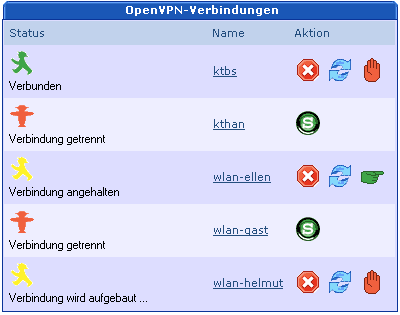
\includegraphics[width=400pt]{verbindungen}
    \caption{Connection Overview}
    \label{fig:guiact}
  \end{figure}

\begin{description}
\item [Status:] State of a connection is symbolized by traffic light symbols. 
  A red man means no OpenVPN process is running a yellow man means  the 
  process is running but no connection could be established (yet) and a 
  green man means that a remote station is \glqq{}connected\grqq{}.
  Details about the connection can be displayed as tool tips for the men. 
  This can be of interest at least for \glqq{}yellow\grqq{} status.
  
\item [Name:] In this column the name of the OpenVPN connection is displayed 
  as defined in configuration. A click on the name leads to an overview showing 
  more informations concerning the connection. See below for details.

\item [Aktion:] The actions provided are symbolized by buttons with a small 
  definition of each realized by a tool tip. These buttons exist:

  \begin{table}[!h]
    \begin{tabular}{lp{12cm}}
      Symbol                                         & Description \\
      \hline\\
      
\includegraphics[width=24pt]{start}            & restart OpenVPN process and try to connect.\\
      
\includegraphics[width=24pt]{stop}             & stop OpenVPN process. \\
      
\includegraphics[width=24pt]{reload}           & reset connection. \\
      
\includegraphics[width=24pt]{hold}             & reset connection and put it in 'hold'. No data can be transferrred. \\
      
\includegraphics[width=24pt]{release}          & free connection again. Data can be transferrred. \\
      \hline\\
    \end{tabular}
  \caption{Actions of the OpenVPN-Webgui}
\end{table}
\end{description} 


\subsubsection{OpenVPN - WebGUI - Detail View Of A Connection}
  \begin{figure}[!h]
    \centering
    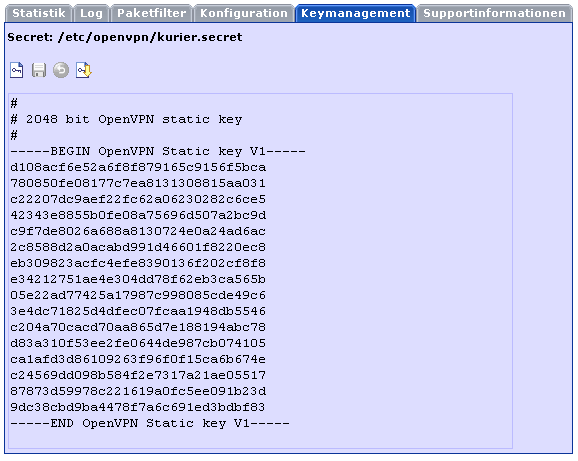
\includegraphics[width=400pt]{detail}
    \caption{Detail view of a connection (Keymanagement)}
    \label{fig:guidetail}
  \end{figure}

\begin{description}
\item [Statistics:] Some interesting statistics are shown here 
    if the connection is started and not on 'hold'.
    
\item [Log:] last 20 lines of the connection logfile. If more lines 
    should be displayed enter the number and click 'show'. If 'all' 
    is selected the whole logfile will be shown. This tab is only shown 
    for started connections.
    
\item [Debug-Log:] Shows the output of the start process. OpenVPN 
    connections are started and the output is shown. This is handy if 
    the connection can't be started by the start button and no normal log 
    can be shown. This tab is only shown for connections not started.

\item [Packet filter:] Shows the configuration of the the packet filter 
    relevant to this connection. Packet filter is only configured 
    if the connection is started and configured as a tunnel.
    
\item [Bridge:] Shows the configuration of bridges on the router. 
    Tab is only shown if the connection is configured as a bridge.
    
\item [Configuration:] Shows the configuration generated on boot for 
    this connection.
    
\item [Keymanagement:] Creates a key for the connection and makes 
    it available for download (see figure \ref{fig:guidetail}). If no 
    key is present on first start it will be generated and displayed 
    automatically. You may download it via the corresponding symbol 
    or copy/paste it to a text file. To save a newly generated keyfile 
    on the router click the disk symbol. Saving can be undone by 
    clicking the restore symbol.

\item [Support informations:] Shows all informations relevant when 
    problems occur.  You may copy\&paste these informations i.e. 
    for a post on the newsgroups.
    
\end{description}


\subsection{OpenVPN - Collaboration Of Different OpenVPN Versions}

Please note that different versions of OpenVPN may use different default 
parameters for a connection. In particular MTU fragment and MSSFIX 
settings may differ. If values \glqq{}don't match\grqq{} connection 
establishment is not possible or no reliable connection can be made. 
Typical error messages can be:

\begin{example}
\begin{verbatim}
FRAG_IN error flags=0xfa2a187b: FRAG_TEST not implemented
FRAG_IN error flags=0xfa287f34: spurrious FRAG_WHOLE flags
\end{verbatim}
\end{example}

Crucial parameters for a connection are:

\begin{description}

\item [OPENVPN\_x\_TUN\_MTU] MTU Values of the TUN device were set to 
  1300 for OpenVPN 1.x. As of OpenVPN 2.0 1500 is the default here.

\item [OPENVPN\_x\_LINK\_MTU] Byte size of the connection in both 
  OpenVPN daemons. The default is depending on OpenVPN Version and 
  operating system version.

\item [OPENVPN\_x\_FRAGMENT] Data packets (UDP or TCP) with a size 
  bigger than the fragment size will be fragmented to packets not 
  bigger than byte size provided in \var{OPENVPN\_x\_FRAGMENT}.

\item [OPENVPN\_x\_MSSFIX] To avoid fragmentation of data packets for 
  TCP connections over VPN a maximum size for TCp data packets can be 
  set here. Up-to-date operating systems will honorate this setting 
  and make fragmentation unnecessary.

\end{description}

Different OpenVPN versions use the following settings as default values. 
Please obey these values when connecting OpenVPN in varying versions.
Default settings on fli4l routers are shown in the second table.

\begin{table}[htbp]
  \begin{scriptsize}
    \begin{tabular}{lll}
      OpenVPN Version/Option        & 1.xx                & 2.00        \\
      \hline                                                    \\
      OPENVPN\_x\_TUN\_MTU          & 1300                & 1500        \\
      OPENVPN\_x\_TUN\_MTU\_EXTRA   & unknown             & 32          \\
      OPENVPN\_x\_FRAGMENT          & unknown             & not configured \\
      OPENVPN\_x\_MSSFIX            & not configured	  & 1450        \\
    \end{tabular}
  \end{scriptsize}
  \caption{Different MTU parameters in different OpenVPN versions.}
\end{table}

\begin{table}[htbp]
  \begin{scriptsize}
    \begin{tabular}{lll}
      fli4l Version/Option          & up to 2.1.8  	  & from 2.1.9 on \\
      \hline                                                    \\
      OPENVPN\_x\_TUN\_MTU          & 1300                & 1500        \\
      OPENVPN\_x\_TUN\_MTU\_EXTRA   & 64                  & 32          \\
      OPENVPN\_x\_FRAGMENT          & not configured	  & 1300        \\
      OPENVPN\_x\_MSSFIX            & not configured	  & 1300        \\
    \end{tabular}
  \end{scriptsize}
  \caption{Different MTU parameters in different fli4l router versions.}
\end{table}

Based on this settings the defaults for your network should be determined 
and written to config/openvpn.txt explicitely. These are the best values for 
your tests to start with:

\begin{example}
\begin{verbatim}
OPENVPN_DEFAULT_TUN_MTU='1500'
OPENVPN_DEFAULT_MSSFIX='1300'
OPENVPN_DEFAULT_FRAGMENT='1300'
\end{verbatim}
\end{example}

For fli4l versions prior to 2.1.9 \glqq{}tun-mtu\grqq{} parameters 
can't be specified directly. But they can be influenced indirectly 
with \var{OPENVPN\_x\_LINK\_MTU}. tun-mtu values are about 45 byte 
smaller than the values in \var{OPENVPN\_x\_LINK\_MTU}. To get exact 
values only trying will help.

\subsection{OpenVPN - Examples}

Some examples will clarify the configuration of package OpenVPN.

\subsubsection{Example - Joining Two Nets Using fli4l Routers}

In the first example two fli4l routers will be connected. Nets behind 
each fli4l router should gain access to each other. Peter and Maria want 
to connect their nets over their fli4l routers. Peter uses a private net 
192.168.145.0/24 and a DynDNS address 'peter.eisfair.net'. Marias setup 
is similar while she is using 10.23.17.0/24 and DynDNS address 
'maria.eisfair.net'. Both trust in each other so they allow unlimited 
access to their complete nets for each other.

\begin{table}[htbp]
  \begin{scriptsize}
    \begin{tabular}{lll}
      OpenVPN Option                & Peter              & Maria               \\
      \hline \\
      OPENVPN\_1\_NAME=             & 'maria'            & 'peter'             \\
      OPENVPN\_1\_REMOTE\_HOST=     & 'maria.eisfair.net' & 'peter.eisfair.net' \\
      OPENVPN\_1\_REMOTE\_PORT=     & '10000'            & '10001'             \\
      OPENVPN\_1\_LOCAL\_PORT=      & '10001'            & '10000'             \\
      OPENVPN\_1\_SECRET=           & 'pema.secret'      & 'pema.secret'       \\
      OPENVPN\_1\_TYPE=             & 'tunnel'           & 'tunnel'            \\
      OPENVPN\_1\_REMOTE\_VPN\_IP=  & '192.168.200.202'  & '192.168.200.193'   \\
      OPENVPN\_1\_LOCAL\_VPN\_IP=   & '192.168.200.193'  & '192.168.200.202'   \\
      OPENVPN\_1\_ROUTE\_N=         & '1'                & '1'                 \\
      OPENVPN\_1\_ROUTE\_1=         & '10.23.17.0/24'    & '192.168.145.0/24'  \\
      OPENVPN\_1\_PF\_INPUT\_N=   & '1'                & '1'                 \\
      OPENVPN\_1\_PF\_INPUT\_1=   & 'ACCEPT'           & 'ACCEPT'            \\
      OPENVPN\_1\_PF\_FORWARD\_N= & '1'                & '1'                 \\
      OPENVPN\_1\_PF\_FORWARD\_1= & 'ACCEPT'  & 'ACCEPT' \\
    \end{tabular}
  \end{scriptsize}
  \caption{OpenVPN Configuration with 2 fli4l routers}
\end{table}

\subsubsection{Example - Two Nets Connected By A Bridge}

In the next example a bridge over a wi-fi connection will be configured. 
Packet filters are not of use here because usually ethernet frames will be 
forwarded but no IP packets. Please remember that with a bridge a common 
net is used. Thus no IP address can exist twice.

\begin{table}[htbp]
  \begin{scriptsize}
    \begin{tabular}{lll}
      OpenVPN Option           & Peter           & Maria           \\
      \hline \\
      OPENVPN\_2\_NAME         & 'bridge'        & 'bridge'          \\
      OPENVPN\_2\_REMOTE\_HOST & '10.1.0.1'      & '10.2.0.1'      \\
      OPENVPN\_2\_REMOTE\_PORT & '10005'         & '10006'         \\
      OPENVPN\_2\_LOCAL\_HOST  & '10.2.0.1'      & '10.1.0.1'      \\
      OPENVPN\_2\_LOCAL\_PORT  & '10006'         & '10005'         \\
      OPENVPN\_2\_FLOAT        & 'no'            & 'no'            \\
      OPENVPN\_2\_RESTART      & 'never'         & 'never'         \\
      OPENVPN\_2\_SECRET       & 'bridge.secret' & 'bridge.secret' \\
      OPENVPN\_2\_TYPE         & 'bridge'        & 'bridge'        \\
      OPENVPN\_2\_BRIDGE       & 'pema-br'       & 'pema-br'       \\
    \end{tabular}
  \end{scriptsize}
  \caption{OpenVPN Configuration with 2 fli4l routers bridging nets over a wi-fi connection.}
\end{table}

In addition to the settings for OpenVPN a bridge has to be configured 
in advanced\_networking and base.txt has to be adapted to use the bridge device 
and not eth0 as the network device for the internal net. See the relevant 
entries in advanced\_networking's and base's configuration files:

\begin{table}[htbp]
  \begin{scriptsize}
    \begin{tabular}{lll}
      advanced\_networking Option  & Peter           & Maria       \\
      \hline \\
      OPT\_BRIDGE\_DEV             & 'yes'           & 'yes'       \\
      BRIDGE\_DEV\_BOOTDELAY       & 'no'            & 'no'        \\
      BRIDGE\_DEV\_N               & '1'             & '1'         \\
      BRIDGE\_DEV\_1\_NAME         & 'pema-br'       & 'pema-br'   \\
      BRIDGE\_DEV\_1\_DEVNAME      & 'br0'           & 'br0'       \\
      BRIDGE\_DEV\_1\_DEV\_N       & '1'             & '1'         \\
      BRIDGE\_DEV\_1\_DEV\_1\_DEV  & 'eth0'          & 'eth0'      \\
    \end{tabular}
  \end{scriptsize}
  \caption{OpenVPN Configuration with 2 fli4l routers bridging nets over a wi-fi connection. Bridge configuration in advanced\_networking.}
\end{table}

\begin{table}[htbp]
  \begin{scriptsize}
    \begin{tabular}{lll}
      base Option  & Peter           & Maria       \\
      \hline \\
      IP\_NET\_N            & '1'                   & '1'                    \\
      IP\_NET\_1            & '192.168.193.254/24'  & '192.168.193.1/24'     \\
      IP\_NET\_1\_DEV       & 'br0'                 & 'br0'                  \\
    \end{tabular}
  \end{scriptsize}
  \caption{OpenVPN Configuration with 2 fli4l routers bridging nets over a wi-fi connection. Bridge configuration in base.txt.}
\end{table}

\subsubsection{Example - Configure Access For A Road Warrior}

\marklabel{roadwarrior}For this example (Roadwarrior) access to a LAN 
behind fli4l should be configured for a notebook with Windows XP over GPRS. 
OpenVPN is installed on the notebook and the *.ovpn file is edited.  
Unfortunately the tun/tap driver for Windows is not as flexible as its 
Unix pendant. Point-to-Point addresses for VPN IP have to be in a 
255.255.255.252 (or /30) net. If the road warrior should only access 
services in the LAN behind or on the fli4l router itself and does not 
have to be accessed by itself a route on fli4l's side is not necessary. 
The road warrior can be addressed on its virtual IP address 
(\var{OPENVPN\_3\_REMOTE\_VPN\_IP}) if necessary. If the road warrior 
has a fixed IP address a host route could be added if needed. If the 
road warrior i.e. has fixed IP address 192.168.33.33 you could simply 
add the following to fli4l's openvpn.txt:

\begin{example}
\begin{verbatim}
OPENVPN_3_ROUTE_N='1'
OPENVPN_3_ROUTE_1='192.168.33.33/32'
\end{verbatim}
\end{example}

With the configuration of the packet filter shown here complete 
communication in both directions is allowed. Only the fli4l router 
is not directly accessible for the road warrior. That would be 
needed if the road warrior should use the DNS server on the fli4l 
router.

\begin{example}
\begin{verbatim}
OPENVPN_3_PF_FORWARD_N='1'
OPENVPN_3_PF_FORWARD_1='ACCEPT'
\end{verbatim}
\end{example}

For allowing access to fli4l's internal DNS server add the 
following to the configuration of fli4l:

\begin{example}
\begin{verbatim}
OPENVPN_3_PF_INPUT_N='1'
OPENVPN_3_PF_INPUT_1='if:VPNDEV:any tmpl:dns ACCEPT'
\end{verbatim}
\end{example}

\begin{table}[htbp]
  \begin{scriptsize}
    \begin{tabular}{ll}
      OpenVPN Option fli4l router                   & roadwarrior           \\
      \hline \\
      OPENVPN\_3\_NAME='roadwarrior'                & remote peter.eisfair.net \\
      OPENVPN\_3\_LOCAL\_PORT='10011'               & rport 10011 \\
      OPENVPN\_3\_SECRET='roadwarrior.secret'       & secret roadwarrior.secret \\
      OPENVPN\_3\_TYPE='tunnel'                     & dev tun \\
      OPENVPN\_3\_REMOTE\_VPN\_IP='192.168.200.238' & ~ \\
      OPENVPN\_3\_LOCAL\_VPN\_IP='192.168.200.237'  & ifconfig 192.168.200.238 192.168.200.237 \\
      OPENVPN\_3\_ROUTE\_N='0'                      & ~ \\
      OPENVPN\_3\_PF\_FORWARD\_N='1'              & ~ \\
      OPENVPN\_3\_PF\_FORWARD\_1='ACCEPT' & ~ \\
      ~                                             & route 192.168.145.0 255.255.255.0 \\
      ~                                             & comp-lzo \\
      ~                                             & persist-tun \\
      ~                                             & persist-key \\
      ~                                             & ping-timer-rem \\
      ~                                             & ping-restart 60 \\
      ~                                             & proto udp4 \\
      ~                                             & tun-mtu 1500 \\
      ~                                             & fragment 1300 \\
      ~                                             & mssfix \\
    \end{tabular}
  \end{scriptsize}
  \caption{OpenVPN Configuration with a Windows Computer over GPRS.}
\end{table}

\subsubsection{Example - Secure A WLAN Connection}

In this example a WLAN connection will be secured by the help of OpenVPN.
The fli4l router has a LAN and a WLAN card it uses or an access point is 
connected to an additional fli4l NIC. This aims at WLAN clients only 
having access to the VPN port without establishing a VPN connection. 
After connecting succesfully to OpenVPN they should have unlimited 
access with cable nets. DNSMASQ DHCP server's settings have to be 
changed to achieve that. Package advanced\_networking will be needed 
as well. Settings in base.txt:
\var{IP\_NET\_1} is the cable LAN and \var{IP\_NET\_2} is the WLAN.
\begin{example}
\begin{verbatim}
IP_NET_N='2'
IP_NET_1='192.168.3.254/24'
IP_NET_1_DEV='br0'
IP_NET_2='192.168.4.254/24'
IP_NET_2_DEV='eth2'
\end{verbatim}
\end{example}

Set DHCP range to suit your needs.  For \var{IP\_NET\_2}
two settings are mandatory:

\begin{example}
\begin{verbatim}
DHCP_RANGE_2_DNS_SERVER1='none'  
DHCP_RANGE_2_NTP_SERVER='none'  
DHCP_RANGE_2_GATEWAY='none' 
\end{verbatim}
\end{example}

Settings in advanced\_networking.txt:
\begin{example}
\begin{verbatim}
OPT_BRIDGE_DEV='yes'
BRIDGE_DEV_BOOTDELAY='yes'
BRIDGE_DEV_N='1'
BRIDGE_DEV_1_NAME='br'
BRIDGE_DEV_1_DEVNAME='br0'
BRIDGE_DEV_1_DEV_N='1'
BRIDGE_DEV_1_DEV_1_DEV='eth0'
\end{verbatim}
\end{example}

\begin{table}[htbp]
  \begin{scriptsize}
    \begin{tabular}{ll}
      OpenVPN Option Router                         & WLAN-Client         \\
      \hline \\
      OPENVPN\_4\_NAME='wlan1'                      & ~ \\
      OPENVPN\_4\_LOCAL\_HOST='192.168.4.254'       & remote 192.168.4.254\\
      OPENVPN\_4\_LOCAL\_PORT='20001'               & rport 20001 \\
      OPENVPN\_4\_SECRET='wlan1.secret'             & secret wlan1.secret \\
      OPENVPN\_4\_TYPE='bridge'                     & dev tap\\
      OPENVPN\_4\_BRIDGE='br'                       & ~\\
      OPENVPN\_4\_RESTART='never'                   & ~\\
      OPENVPN\_4\_MUTE\_REPLAY\_WARNINGS='yes'      & ~\\
      ~                                             & comp-lzo \\
      ~                                             & persist-tun \\
      ~                                             & persist-key \\
      ~                                             & ping-timer-rem \\
      ~                                             & ping-restart 60 \\
      ~                                             & proto udp4 \\
      ~                                             & tun-mtu 1500 \\
      ~                                             & fragment 1300 \\
      ~                                             & mssfix \\
    \end{tabular}
  \end{scriptsize}
  \caption{OpenVPN Securing a WLAN.}
\end{table}

\subsection{Additional Links On OpenVPN}

At the end here are some links on OpenVPN configuration:

\noindent \altlink{http://openvpn.net} \\
\altlink{http://de.wikipedia.org/wiki/OpenVPN} \\
\altlink{http://openvpn.se/} \\
\altlink{http://arnowelzel.de/wiki/de/fli4l/openvpn} \\
\altlink{http://wiki.freifunk.net/OpenVPN} \\
\altlink{http://w3.linux-magazine.com/issue/24/Charly.pdf} \\
\altlink{http://w3.linux-magazine.com/issue/25/WirelessLAN_Intro.pdf} \\
\altlink{http://w3.linux-magazine.com/issue/25/OpenVPN.pdf} \\
